\documentclass[12pt]{article}
\usepackage{graphicx}
\usepackage{subcaption}
\usepackage[a4paper, margin=2cm]{geometry}
\usepackage{tikz}
\usetikzlibrary{positioning}
\usetikzlibrary{arrows.meta}
\usetikzlibrary{decorations.markings}
\usepackage{pgfplots}
\usepgfplotslibrary{fillbetween}
\pgfplotsset{compat=newest}
\definecolor{matplotlibBlue}{RGB}{31, 119, 191}  
\definecolor{matplotlibOrange}{RGB}{255, 127, 14}  
\definecolor{matplotlibGreen}{RGB}{44, 160, 44}  
\begin{document}

\section{Markov Chain Diagrams}

\begin{figure}[h!]
    \centering
    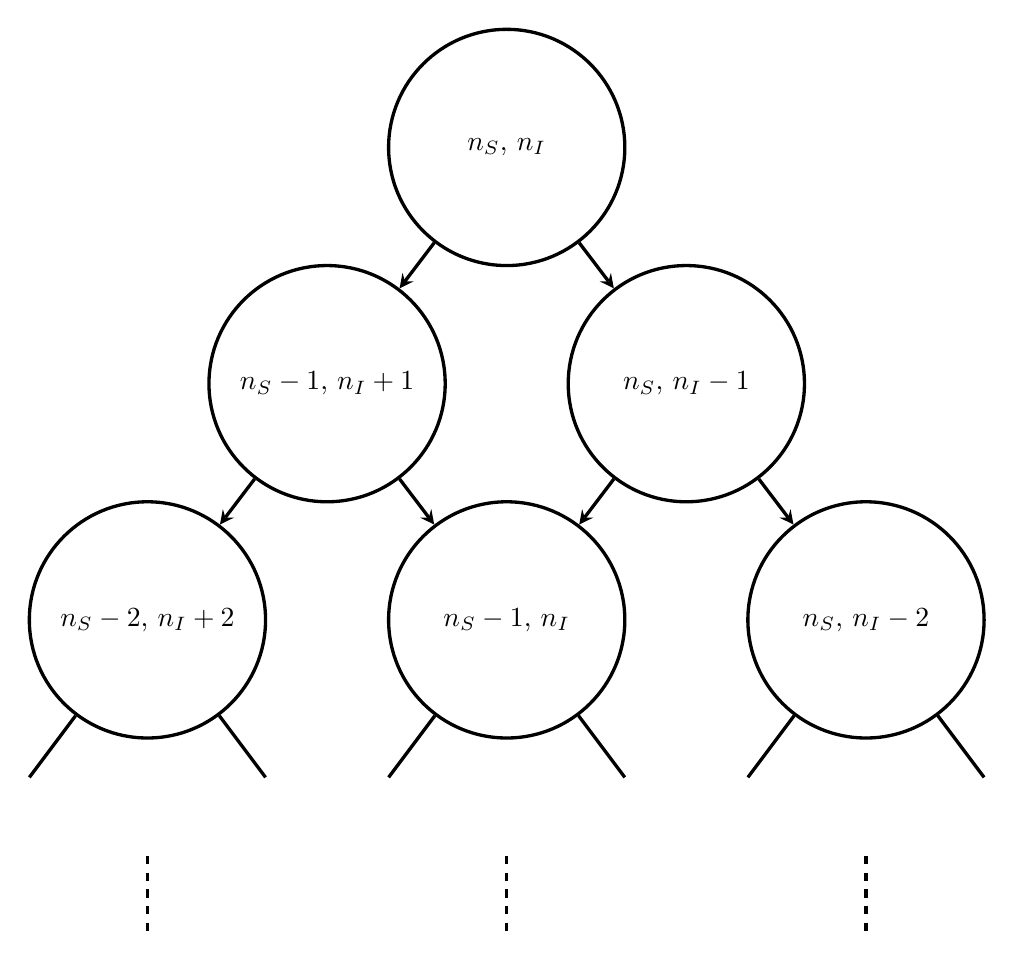
\begin{tikzpicture}[
        roundnode/.style={circle, draw=black, fill=white, very thick, minimum size=3cm}, % effective page width is L-a
    ]
    
    % Objects
    \node[roundnode] (tauZero) at (0.5\linewidth-1.5cm,0) {$n_S$, $n_I$};
    \node[roundnode] (tauOneOptionOne) at (0.25\linewidth-0.75cm,-3cm) {$n_S-1$, $n_I+1$};
    \node[roundnode] (tauOneOptionTwo) at (0.75\linewidth-2.25cm,-3cm) {$n_S$, $n_I-1$};
    \node[roundnode] (tauTwoOptionOne) at (0,-6cm) {$n_S-2$, $n_I+2$};
    \node[roundnode] (tauTwoOptionTwo) at (0.5\linewidth-1.5cm,-6cm) {$n_S-1$, $n_I$};
    \node[roundnode] (tauTwoOptionThree) at (\linewidth-3cm,-6cm) {$n_S$, $n_I-2$};
    
    % Lines
    \draw[very thick,-stealth] (tauZero) -- (tauOneOptionOne);
    \draw[very thick,-stealth] (tauZero) -- (tauOneOptionTwo);
    \draw[very thick,-stealth] (tauOneOptionOne) -- (tauTwoOptionOne);
    \draw[very thick,-stealth] (tauOneOptionOne) -- (tauTwoOptionTwo);
    \draw[very thick,-stealth] (tauOneOptionTwo) -- (tauTwoOptionTwo);
    \draw[very thick,-stealth] (tauOneOptionTwo) -- (tauTwoOptionThree);
    \draw[very thick,-] (tauTwoOptionOne) -- (-1.5cm, -8cm);
    \draw[very thick,-] (tauTwoOptionOne) -- (1.5cm, -8cm);
    \draw[very thick,-] (tauTwoOptionTwo) -- (0.5\linewidth-3cm, -8cm);
    \draw[very thick,-] (tauTwoOptionTwo) -- (0.5\linewidth, -8cm);
    \draw[very thick,-] (tauTwoOptionThree) -- (\linewidth-4.5cm, -8cm);
    \draw[very thick,-] (tauTwoOptionThree) -- (\linewidth-1.5cm, -8cm);
    
    \draw[very thick,dashed] (0, -9cm) -- (0, -10cm);
    \draw[very thick,dashed] (0.5\linewidth-1.5cm, -9cm) -- (0.5\linewidth-1.5cm, -10cm);
    \draw[very thick,dashed] (\linewidth-3cm, -9cm) -- (\linewidth-3cm, -10cm);
    
    \end{tikzpicture}
    
\end{figure}

%%%%%%%%%%%%%%%%%%%%%%%%%%%%%%%%%%%%%%%%%%%%%%%%%%%%%%%%%%%%%%
\newpage

\begin{figure}[h!]
    \centering

    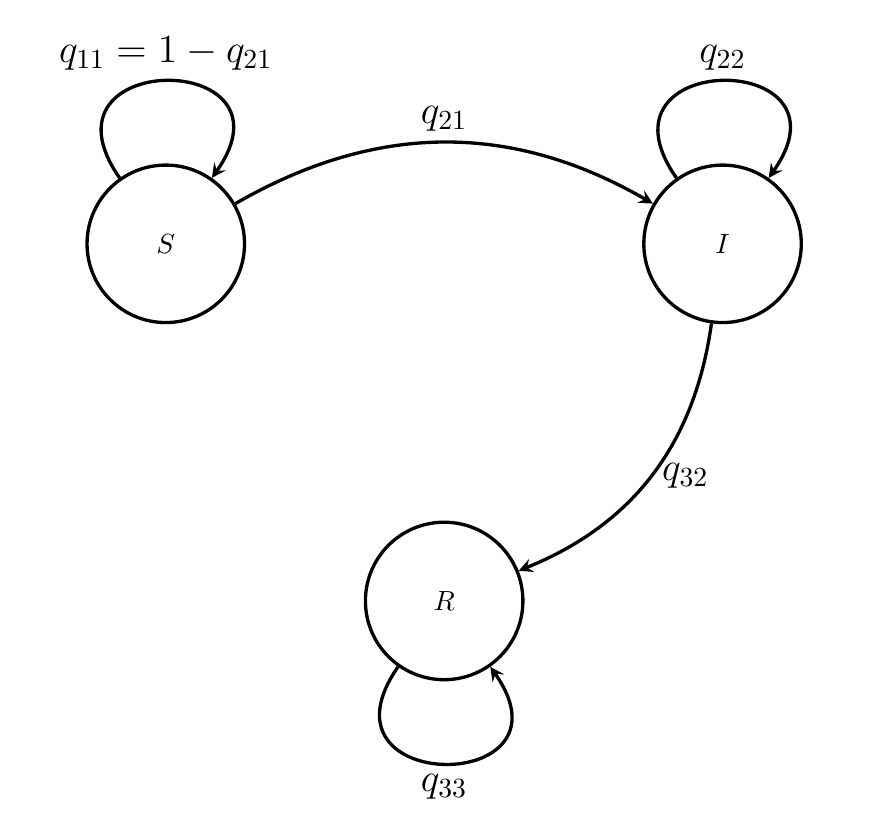
\begin{tikzpicture}[
        >=stealth,
        node distance=5cm,
        roundnode/.style={circle, draw=black, very thick, minimum size=2cm}
    ]
    
        \node [roundnode] (State1) {$S$};
        \node [roundnode] (State3) [below right of= State1, yshift=-1cm] {$R$};
        \node [roundnode] (State2) [above right of= State3, yshift=1cm] {$I$};

        \path[->,very thick] (State1) edge [ bend left ] node [ above ] {\Large $q_{21}$} (State2) ;
        \path[->,very thick] (State1) edge [ loop above, out=125,in=55,distance=2cm ] node [ above ] {\Large $q_{11} = 1 - q_{21}$} (State1) ;
        \path[->,very thick] (State2) edge [ loop above, out=125,in=55,distance=2cm ] node [ above ] {\Large $q_{22}$} (State2) ;
        \path[->,very thick] (State2) edge [ bend left ] node [ right ] {\Large $q_{32}$} (State3) ;
        \path[->,very thick] (State3) edge [ loop below, out=-125,in=-55,distance=2cm ] node [ below ] {\Large $q_{33}$} (State3) ;
        
    \end{tikzpicture}

\end{figure}

\begin{figure}[h!]
    \centering

    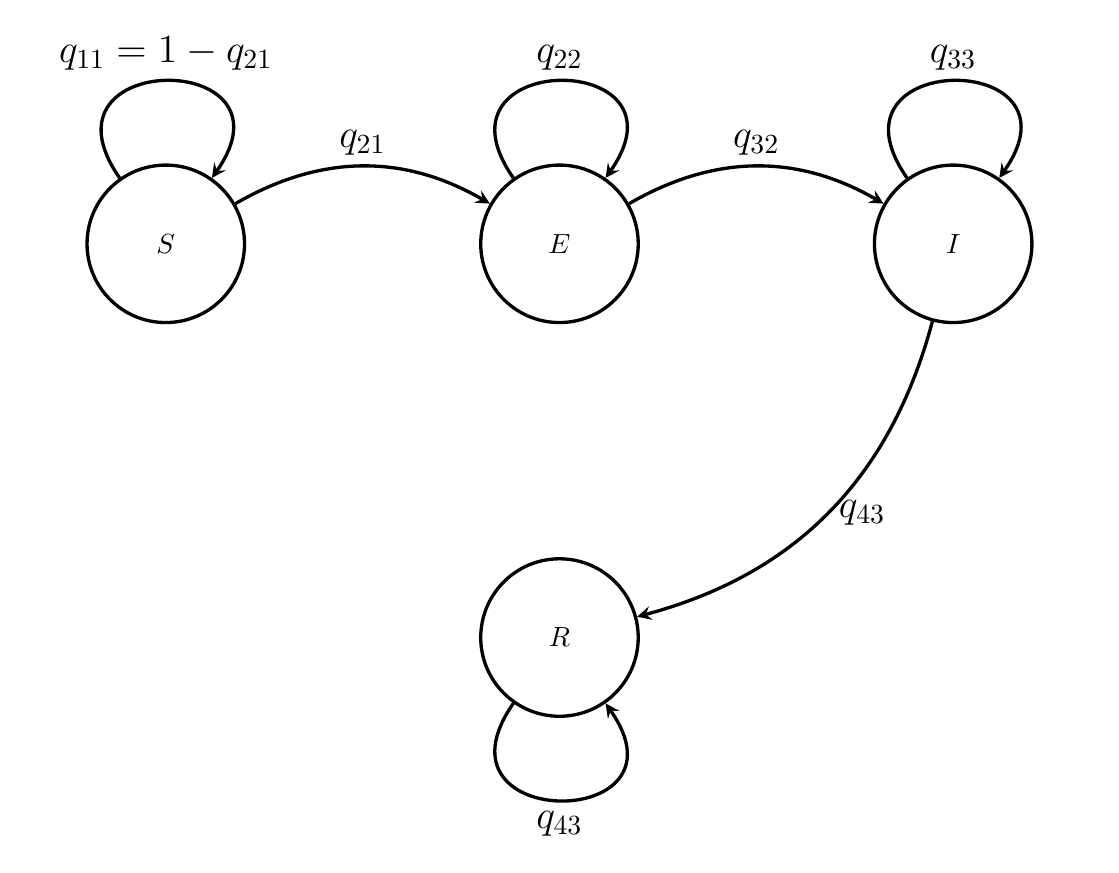
\begin{tikzpicture}[
        >=stealth,
        node distance=5cm,
        roundnode/.style={circle, draw=black, very thick, minimum size=2cm}
    ]
    
        \node [roundnode] (State1) {$S$};
        \node [roundnode] (State2) [right of= State1] {$E$};
        \node [roundnode] (State3) [right of= State2] {$I$};
        \node [roundnode] (State4) [below of= State2] {$R$};

        \path[->,very thick] (State1) edge [ bend left ] node [ above ] {\Large $q_{21}$} (State2) ;
        \path[->,very thick] (State1) edge [ loop above, out=125,in=55,distance=2cm ] node [ above ] {\Large $q_{11} = 1 - q_{21}$} (State1) ;
        \path[->,very thick] (State2) edge [ bend left ] node [ above ] {\Large $q_{32}$} (State3) ;
        \path[->,very thick] (State2) edge [ loop above, out=125,in=55,distance=2cm ] node [ above ] {\Large $q_{22}$} (State2) ;
        \path[->,very thick] (State3) edge [ bend left ] node [ right ] {\Large $q_{43}$} (State4) ;
        \path[->,very thick] (State3) edge [ loop above, out=125,in=55,distance=2cm ] node [ above ] {\Large $q_{33}$} (State3) ;
        \path[->,very thick] (State4) edge [ loop below, out=-125,in=-55,distance=2cm ] node [ below ] {\Large $q_{43}$} (State4) ;
        
    \end{tikzpicture}

\end{figure}

%%%%%%%%%%%%%%%%%%%%%%%%%%%%%%%%%%%%%%%%%%%%%%%%%%%%%%%%%%%%%%
\newpage

\begin{figure}[h!]
    \centering
    \begin{tikzpicture}[
        >=stealth,
        node distance=7cm,
        roundnode/.style={circle, draw=black, very thick, minimum size=3cm}
    ]

        \node [roundnode] (State0) {$n_x,\ n_y$};
        \node [roundnode] (State1) [left of = State0] {$n_x-1,\ n_y$};
        \node [roundnode] (State2) [above of = State0] {$n_x,\ n_y-1$};
        \node [roundnode] (State3) [right of = State0] {$n_x+1,\ n_y$};
        \node [roundnode] (State4) [below of = State0] {$n_x,\ n_y+1$};

        % Arrows from centre outwards
        \path[->,very thick] (State0) edge [ bend left ] node [ below ] {$p(n_x,\ n_y \rightarrow n_x-1,\ n_y)$} (State1) ;
        \path[->,very thick] (State0) edge [ bend left ] node [ left ] {$p(n_x,\ n_y \rightarrow n_x,\ n_y-1)$} (State2) ;
        \path[->,very thick] (State0) edge [ bend left ] node [ above ] {$p(n_x,\ n_y \rightarrow n_x+1,\ n_y)$} (State3) ;
        \path[->,very thick] (State0) edge [ bend left = 60] node [ right ] {$p(n_x,\ n_y \rightarrow n_x,\ n_y+1)$} (State4) ;

        % Self Loop
        \path[->,very thick] (State0) edge [ loop below, out=-120,in=-55,distance=2cm ] node [ below ] {$p(n_x,\ n_y \rightarrow n_x,\ n_y)$} (State0) ;
        
    \end{tikzpicture}

\end{figure}

%%%%%%%%%%%%%%%%%%%%%%%%%%%%%%%%%%%%%%%%%%%%%%%%%%%%%%%%%%%%%%
\newpage
\section{Plots}
% Helpful youtube video: https://youtu.be/5jmIHOWpEg0?si=NlE917YHjn-7zVWx

\begin{figure}[h!]
\begin{subfigure}{.5\linewidth}
    \centering
    \begin{tikzpicture}
    \node at (0.3,5.45) {(a)};
    \begin{axis}[
        enlarge x limits=false,
        xlabel = $t$ (days),
        ylabel = No. People,
        ylabel near ticks,
        ]  
    
        \addplot+[color=matplotlibBlue,mark=none,line width=1pt]
        table[x=Time,y=Susceptible,col sep=comma]
        {SIRmicroscopic1.txt};
        \addplot+[color=matplotlibOrange,mark=none,line width=1pt]
        table[x=Time,y=Infected,col sep=comma]
        {SIRmicroscopic1.txt};
        \addplot+[color=matplotlibGreen,mark=none,line width=1pt]
        table[x=Time,y=Recovered,col sep=comma]
        {SIRmicroscopic1.txt};
    
    \end{axis}
    \end{tikzpicture}
    \label{fig:sfig1}
\end{subfigure}%
\hspace{1cm}
\begin{subfigure}{.5\linewidth}
    \centering
    \begin{tikzpicture}
    \node at (0.3,5.45) {(b)};
    \begin{axis}[
        enlarge x limits=false,
        xlabel = $t$ (days),
        yticklabel=\empty
        ]    
    
        \addplot [color=matplotlibBlue,mark=none,line width=1pt]
        table[x=Time,y=Susceptible,col sep=comma]
        {SIRmicroscopic2.txt};
        \addplot [color=matplotlibOrange,mark=none,line width=1pt]
        table[x=Time,y=Infected,col sep=comma]
        {SIRmicroscopic2.txt};
        \addplot [color=matplotlibGreen,mark=none,line width=1pt]
        table[x=Time,y=Recovered,col sep=comma]
        {SIRmicroscopic2.txt};
    \end{axis}
    \end{tikzpicture}
    \label{fig:sfig2}
\end{subfigure}
\caption{Microscopic SIR model with 100,000 people. System starts from 1 infection and 99,999 susceptible.}
\label{fig:fig}
\end{figure}
%%%%%%%%%%%%%%%%%%%%%%%%%%%%%%%%%%%%%%%%%%%%%%%%%%%%%%%%%%%%%%
\begin{figure}
\begin{center}
\pgfplotslegendfromname{namedLegendMacroscopicSIR}
\end{center}

\begin{subfigure}{.5\linewidth}
    \centering
    \begin{tikzpicture}
    \node at (1,5.45) {(a) $\beta=3$};
    \begin{axis}[
        legend columns=3,
        legend entries={Susceptible,Infected,Recovered},
        legend to name=namedLegendMacroscopicSIR,
        enlarge x limits=false,
        xlabel = $t$ (days),
        ylabel = No. People,
        ylabel near ticks,
    ]
        \addplot+[color=matplotlibBlue,mark=none,line width=1pt]
        table[x=Time,y=Susceptible,col sep=comma]{SIRmacroscopicBeta3.txt};
        \addplot+[color=matplotlibOrange,mark=none,line width=1pt]
        table[x=Time,y=Infected,col sep=comma]{SIRmacroscopicBeta3.txt};
        \addplot+[color=matplotlibGreen,mark=none,line width=1pt]
        table[x=Time,y=Recovered,col sep=comma]{SIRmacroscopicBeta3.txt};
    \end{axis}
    \end{tikzpicture}
\end{subfigure}
\begin{subfigure}{.5\linewidth}
    \centering
    \begin{tikzpicture}
    \node at (1,5.45) {(b) $\beta=7$};
    \begin{axis}[
        enlarge x limits=false,
        xlabel = $t$ (days),
        yticklabel=\empty,
    ]
        \addplot[color=matplotlibBlue,mark=none,line width=1pt]
        table[x=Time,y=Susceptible,col sep=comma]{SIRmacroscopicBeta7.txt};
        \addplot[color=matplotlibOrange,mark=none,line width=1pt]
        table[x=Time,y=Infected,col sep=comma]{SIRmacroscopicBeta7.txt};
        \addplot[color=matplotlibGreen,mark=none,line width=1pt]
        table[x=Time,y=Recovered,col sep=comma]{SIRmacroscopicBeta7.txt};
    \end{axis}
    \end{tikzpicture}
\end{subfigure}

\caption{SIR model with $\beta/N$ people infected per day per infected person per susceptible person and $\gamma$ people recovered per day per infected person, where $N$ is the total population. (a): $\beta=3$, $\gamma=1$; (b): $\beta=7$, $\gamma=1$. Figures produced by M. G. Hauge Evans.}
\label{fig:macroscopicSIR}
\end{figure}

%%%%%%%%%%%%%%%%%%%%%%%%%%%%%%%%%%%%%%%%%%%%%%%%%%%%%%%%%%%%%%

\begin{figure}
\begin{center}
\pgfplotslegendfromname{namedLegendMacroscopicSIREnsemble}
\end{center}
\begin{subfigure}{.5\linewidth}
    \centering
    \begin{tikzpicture}
    \node at (2,5.3) {(a) $\beta=7,I_0=1$};
    \begin{axis}[
        enlarge x limits=false,
        xlabel = $t$ (days),
        ylabel = No. People,
        ylabel near ticks,
        ]   
        \addplot [color=matplotlibBlue,mark=none,line width=1pt]
        table[x=time,y=state1Mean,col sep=comma]
        {SIRensembleSusceptibleBeta7I1.txt};
        \addplot [name path=susceptible_top,color=matplotlibBlue,mark=none,line width=0pt]
        table[x=time,y=state1upper,col sep=comma]
        {SIRensembleSusceptibleBeta7I1.txt};
        \addplot [name path=susceptible_bottom,color=matplotlibBlue,mark=none,line width=0pt]
        table[x=time,y=state1lower,col sep=comma]
        {SIRensembleSusceptibleBeta7I1.txt};
        \addplot[matplotlibBlue!50,fill opacity=0.5] fill between[of=susceptible_top and susceptible_bottom];

	\addplot [color=matplotlibOrange,mark=none,line width=1pt]
        table[x=time,y=state2Mean,col sep=comma]
        {SIRensembleInfectedBeta7I1.txt};
        \addplot [name path=infected_top,color=matplotlibOrange,mark=none,line width=0pt]
        table[x=time,y=state2upper,col sep=comma]
        {SIRensembleInfectedBeta7I1.txt};
        \addplot [name path=infected_bottom,color=matplotlibOrange,mark=none,line width=0pt]
        table[x=time,y=state2lower,col sep=comma]
        {SIRensembleInfectedBeta7I1.txt};
        \addplot[matplotlibOrange!50,fill opacity=0.5] fill between[of=infected_top and infected_bottom];

	\addplot [color=matplotlibGreen,mark=none,line width=1pt]
        table[x=time,y=state3Mean,col sep=comma]
        {SIRensembleRecoveredBeta7I1.txt};
        \addplot [name path=recovered_top,color=matplotlibGreen,mark=none,line width=0pt]
        table[x=time,y=state3upper,col sep=comma]
        {SIRensembleRecoveredBeta7I1.txt};
        \addplot [name path=recovered_bottom,color=matplotlibGreen,mark=none,line width=0pt]
        table[x=time,y=state3lower,col sep=comma]
        {SIRensembleRecoveredBeta7I1.txt};
        \addplot[matplotlibGreen!50,fill opacity=0.5] fill between[of=recovered_top and recovered_bottom];
    \end{axis}
    \end{tikzpicture}
\end{subfigure}
\begin{subfigure}{.5\linewidth}
    \centering
    \begin{tikzpicture}
    \node at (2,5.3) {(b) $\beta=7,I_0=10$};
    \begin{axis}[
        legend columns=3,
        legend entries={Susceptible,Infected,Recovered},
        legend to name=namedLegendMacroscopicSIREnsemble,
        enlarge x limits=false,
        xlabel = $t$ (days),
        ylabel near ticks,
       ]
        \addplot [color=matplotlibBlue,mark=none,line width=1pt]
        table[x=time,y=state1Mean,col sep=comma]
        {SIRensembleSusceptibleBeta7I10.txt};
        \addplot [color=matplotlibOrange,mark=none,line width=1pt]
        table[x=time,y=state2Mean,col sep=comma]
        {SIRensembleInfectedBeta7I10.txt};
        \addplot [color=matplotlibGreen,mark=none,line width=1pt]
        table[x=time,y=state3Mean,col sep=comma]
        {SIRensembleRecoveredBeta7I10.txt};

        \addplot [name path=susceptible_top,color=matplotlibBlue,mark=none,line width=0pt]
        table[x=time,y=state1upper,col sep=comma]
        {SIRensembleSusceptibleBeta7I10.txt};
        \addplot [name path=susceptible_bottom,color=matplotlibBlue,mark=none,line width=0pt]
        table[x=time,y=state1lower,col sep=comma]
        {SIRensembleSusceptibleBeta7I10.txt};
        \addplot[matplotlibBlue!50,fill opacity=0.5] fill between[of=susceptible_top and susceptible_bottom];

	
        \addplot [name path=infected_top,color=matplotlibOrange,mark=none,line width=0pt]
        table[x=time,y=state2upper,col sep=comma]
        {SIRensembleInfectedBeta7I10.txt};
        \addplot [name path=infected_bottom,color=matplotlibOrange,mark=none,line width=0pt]
        table[x=time,y=state2lower,col sep=comma]
        {SIRensembleInfectedBeta7I10.txt};
        \addplot[matplotlibOrange!50,fill opacity=0.5] fill between[of=infected_top and infected_bottom];

	
        \addplot [name path=recovered_top,color=matplotlibGreen,mark=none,line width=0pt]
        table[x=time,y=state3upper,col sep=comma]
        {SIRensembleRecoveredBeta7I10.txt};
        \addplot [name path=recovered_bottom,color=matplotlibGreen,mark=none,line width=0pt]
        table[x=time,y=state3lower,col sep=comma]
        {SIRensembleRecoveredBeta7I10.txt};
        \addplot[matplotlibGreen!50,fill opacity=0.5] fill between[of=recovered_top and recovered_bottom];
    \end{axis}
    \end{tikzpicture}
\end{subfigure}
\caption{Ensemble averaged SIR model with $\beta/N$ people infected per day per infected person per susceptible person and $\gamma=1$ people recovered per day per infected person, where $N=100$ is the total population. $I_0$ people are infected at $t=0$ and the rest of the population is susceptible. (a): $\beta=7$, $I_0=1$; (b): $\beta=7$, $I_0=10$. Figures produced by M. G. Hauge Evans.}
\label{fig:macroscopicSIREnsemble}
\end{figure}
%%%%%%%%%%%%%%%%%%%%%%%%%%%%%%%%%%%%%%%%%%%%%%%%%%%%%%%%%%%%%%
\begin{figure}
\centering
\begin{tikzpicture}
\begin{axis}[
	legend columns=3,
      	legend entries={Person 1, Person2},
       	legend to name=namedLegendRandomWalk,
	unit vector ratio*=1 1 1,
        	enlarge x limits=false,
	enlarge y limits=false,
        	xlabel = $x$ (m),
        	ylabel = $y$ (m),
	ylabel near ticks,
	xlabel near ticks,
	xmin=0,
	xmax=50,
	ymin=0, 
	ymax=50
]
	\addplot+[color=matplotlibBlue,mark=none,line width=1pt]
	table[x=position_x,y=position_y,col sep=comma]{person1.txt};
	\addplot+[color=matplotlibOrange,mark=none,line width=1pt]
	table[x=position_x,y=position_y,col sep=comma]{person2.txt};
\end{axis}
\end{tikzpicture}
\caption{Random Walk Plot. Figures produced by M. G. Hauge Evans.}
\label{fig:randomWalkPlot}
\end{figure}
\end{document}
